\documentclass[11pt]{article}

\usepackage{times}
\usepackage{epsfig}
\usepackage{graphicx}
\usepackage{amsmath}
\usepackage{amssymb}
\usepackage{color, soul} 	%for highlighting
\usepackage{listings} 		%for writing code
\lstset{
basicstyle=\small\ttfamily,
columns=flexible,
breaklines=true
}
\usepackage[margin=1in]{geometry} %for margins

\setcounter{page}{1}
\begin{document}

\begin{titlepage}

\title{Space Brain - Implementing a Convolutional Network on an Embedded System with an FPGA for Space Applications Suitability Testing}
\author{Jukka (Jacobus) Hertzog}
\def\supervisor{Dr. Felix Winterstein}
\def\secondmarker{Dr. David Thomas}
\def\course{EE4T}
\def\cid{00828711}

\setlength{\parindent}{0pt}
\setlength{\parskip}{0pt}
\fontfamily{phv}\selectfont
{
\large
\raggedright
Imperial College London\\[17pt]
Department of Electrical and Electronic Engineering\\[17pt]
Final Year Project Interim Report 2017\\[17pt]
}
\rule{\columnwidth}{3pt}
\vfill
\centering
\makeatletter
\begin{tabular}{p{40mm}p{\dimexpr\columnwidth-40mm}}
Project Title: & \textbf{\@title} \\[12pt]
Student: & \textbf{\@author} \\[12pt]
CID: & \textbf{\cid} \\[12pt]
Course: & \textbf{\course} \\[12pt]
Project Supervisor: & \textbf{\supervisor} \\[12pt]
Second Marker: & \textbf{\secondmarker} \\
\end{tabular}
\end{titlepage}

\section{Introduction}
\label{sec:Introduction}

Convolutional Neural Networks (CNNs) are a powerful Deep Learning tool that can be used to solve extremely complex computational problems. In particular, they have gained popularity in computer vision and image classification applications, performing with very high accuracy. However, CNNs are extremely computationally heavy. As a result, implementing them on embedded systems, which typically have very limited resources, presents many challenges. A promising solution to this problem is the use of an FPGA, which provide a very high computational power with low power usage.

Consider a miniature research satellite (a CubeSat), that uses a camera to capture images to be classified. Normally the images would be transmitted to a ground station to be processed, but in this case, channel capacity during the transmission window is too limited and the raw data is too large for this to be feasible, so the idea is to process and classify images on board the satellite and just transmit the results. Therefore, the aim of this project is to implement a CNN on an FPGA-based system, and then to investigate the suitability of this system for space applications.

\section{Project Specification}
\label{sec:ProjSpec}

\subsection{Implementation of a CNN on an FPGA}
\label{sec:ProjSpec-ImplementationOfACNNOnAnFPGA}

The first deliverable is the implementation of a CNN on an embedded platform. The hardware used is a product from Xilinx called a Zedboard, a development board for the Zynq-7000 System On a Chip (SoC). The Zynq-7000 consists of a Xilinx 28nm Artix-7 FPGA and a dual-core Cortex-A9 ARM processor integrated together. The processor, with it's easily developed code, will control the system, while the FPGA, being able to efficiently perform heavy computations, will be used to accelerate functions.

The end result will be a fully functional CNN that runs on the Zedboard and is able to process and classify images with a reasonable execution time and accuracy, compared to implementations from literature discussed in section \ref{sec:Background-CNNsImplementedOnFPGAs}. \hl{possibly different section?}

\subsection{Investigation of Fault Tolerance in the Presence of Bit-stream Corruptions}
\label{sec:ProjSpec-InvestigationOfFaultToleranceInThePresenceOfBitstreamCorruptions}

The second deliverable of this project is the invesitgation of the system's fault tolerance against SEUs. As discussed in section \ref{sec:Background-FPGAsAndSpaceApplications}, SEUs from are one of the main challenges to be overcome when using SRAM based FPGAs for applications in space. The system's resistance to SEUs should indicate whether or not the system might be suitable as an on board processor for a satellite in orbit.

\section{Background}
\label{sec:Background}

\subsection{Convolutional Neural Networks}
\label{sec:Background-CNN}

CNNs can be used to classify images in a forward inference process. But before using the CNN for any task, one should first train the CNN on a dataset. Recent research [15] showed that, a CNN model pre-trained on a large dataset for a given task can be used for other tasks and achieved high accuracy with minor adjustment in network weights. This minor adjustment is called "fine-tune". The training of the CNN is mostly implemented on large servers. For the embedded FPGA platform, we only focus on accelerating the inference process of a CNN, and not on the training process.

A typical CNN consists of a number of layers that run in sequence. The parameters of a CNN model are called "weights". The first layer of a CNN reads an input image and outputs a series of feature maps. The input image will be three dimensional - the height and width of the image make up two dimensions, and colours make up the third layer. For an RGB image, the input will have a depth of 3, while a grayscale image will have a depth of 1. The following layers read the feature maps generated by previous layers and output new feature maps. Finally a classifier outputs the probability of each category that the input image might belong to. Convolution (CONV) layers and Fully Connected (FC) layers are two essential types of layer in CNN. After CONV layers, there are usually pooling layers. A typical CNN example is shown in Figure \ref{fig:typicalCNN}.

\begin{figure}

\centering
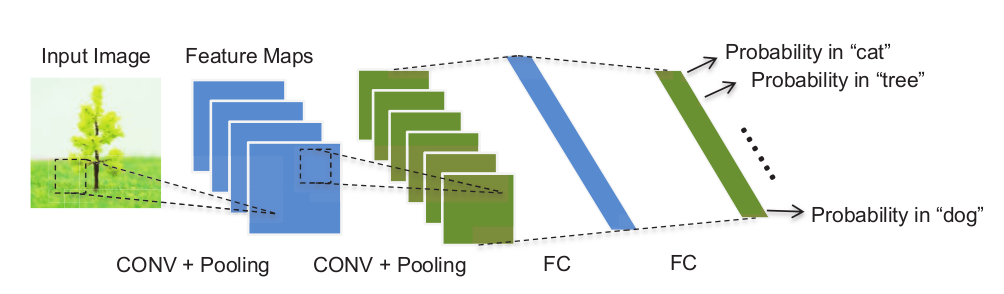
\includegraphics[width=0.75\textwidth]{../figures/typicalCnn}

  \caption{A typical CNN structure from the feature map per
spective \label{fig:typicalCNN}}

\end{figure}

A CNN's structure is comprised of multiple convolutional layers, interspersed by pooling and activation function layers. These convolution layers decompose the input image to different features maps varying from low-level features such as edges, lines, curves, etc., in the initial layers to high-level/abstract features in the deeper layers. These extracted features are classified to output classes by fully-connected classification layers that are similar to multi-layer perceptrons.

\subsubsection{Convolution Layer}
\label{sec:Background-CNN-Conv}

Convolution is the most critical operation of a CNN and it constitutes over 90\% of the total operations in many CNN models. The CONV layer takes a series of feature maps as input and convolves with convolutional kernels to obtain the output feature maps. It involves 3-dimensional multiply and accumulate operation of $N_{if}$ input features with $K\times K$ convolution kernels to get an output feature neuron value as shown in Equation \ref{eq:ConvLayer}.

\begin{equation}
out(f_o,x,y)=\sum^{N_{if}}_{f_i=0} \sum^{K}_{k_x=0} \sum^{K}_{k_y=0} wt(f_o,f_i,k_x,k_y)\times in(f_i,x+k_x,y+k_y)
\label{eq:ConvLayer}
\end{equation}
where $out(f_o,x,y)$ and $in(f_i,x,y)$ represent the neurons at position $(x,y)$ in the feature maps $f_o$ and $f_i$, respectively and $wt(f_o,f_i,k_x,k_y)$ is the weights at position $(k_x,k_y)$ that gets convolved with input feature map $f_i$ to get the output feature map $f_o$.

\subsubsection{Activation Functions}
\label{sec:Background-CNN-Activation}

CONV layers are followed by an activation functon layer. This layer can be thought of as a decision, based on the output of the CONV layer, on to what extent each neuron in the next layer has been activated. The CONV layer output is a linear combination of the inputs and the weights at a position in the network, and role of the activation function is to produce a non-linear decision boundary. The commonly used activation functions in traditional neural networks are non-linear functions such as tanh and sigmoid, which require a longer training time in CNNs \cite{AlexNet}. Hence, Rectified Linear Unit (ReLU), defined as $y = max(x,0)$, has become the popular activation function among CNN models as it converges faster in training, and has less computational complexity than exponent functions in tanh and sigmoid, also aiding hardware design.

\subsubsection{Pooling Layer}
\label{sec:Background-CNN-Pool}

Spatial pooling or subsampling is utilized to reduce the feature dimensions as we traverse deeper into the network. As shown in Equation \ref{eq:Pool}, pooling computes the maximum or average of neighboring $K\times K$ neurons in the same feature map, which also provides a form of translational invariance\cite{PoolAnalysis}. Although max-pooling is popularly used, and average pooling is also used in some CNN models\cite{PoolAnalysis}. Reducing the dimensionality of lower-level features while preserving the important information, the pooling layer helps abstracting higher-level features without redundancy.

\begin{equation}
out(f_o,x,y)=\underset{0\geqslant (k_x,k_y)<K}{max/average}(in(f_o,x+k_x,y+k_y))
\label{eq:Pool}
\end{equation}

\subsubsection{Fully Connected Layer}
\label{sec:Background-CNN-FC}

An FC layer is a classification layer where all the input features $(N_{if})$ are connected to all of the output features $(N_{of})$ through synaptic weights $(wt)$. These are at the end of the CNN and perform the final classification, based on the features that have been recognised by the rest of the network. Each output neuron is the weighted summation of all the input neurons as shown in Equation \ref{eq:FullyConnected}.

\begin{equation}
out(f_o)=\sum^{N_{if}}_{f_i=0}wt(f_o,f_i)\times in(f_i)
\label{eq:FullyConnected}
\end{equation}
The outputs of the inner-product layer traverse through ReLU based activation function to the next inner-product layer or directly to a Softmax function that converts them to probability in the range (0, 1). The final accuracy layer compares the labels of the top probabilities from softmax layer with the actual label and gives the accuracy of the CNN model.

\subsection{CNNs Implemented on FPGAs}
\label{sec:Background-CNNsImplementedOnFPGAs}

\subsection{FPGAs and Space Applications}
\label{sec:Background-FPGAsAndSpaceApplications}

Single Event Upsets (SEUs).

\section{Implementation Plan}
\label{sec:ImpPlan}

\subsection{Infrastrucure Setup}
\label{sec:ImpPlan-InfSetup}

This first part of the project implementation will be setting up two important tools that will be vital during the 

An important tool in this process will be Xilinx's SDSoc development environment. SDSoc is able to optimise and compile C, C++ or OpenCL source code for a Zynq system. The compiler generates software for the ARM core and, using a High Level Synthesis (HLS) tool, a bitstream for the FPGA. This allows the user to design the entire system, easily accelerating functions with the FPGA. SDSoc is a very powerful tool, facilitating the rapid development and design of firmware.

Another important tool will be Caffe (or Convolutional Architecture for Fast Feature Embedding). This is a deep learning framework that can be used to design, train, optimise and test CNNs, with a focus on computer vision\cite{jia2014caffe}. It also includes some examples of pre-trained CNN models that are ready for use. Using Caffe, it will be possible to generate C++ code for a CNN, which can then be implemented on the Zynq system using SDSoc.

\subsection{FPGA Implementation of a CNN}
\label{sec:ImpPlan-FPGAImplOfCnn}

\subsection{Fault Injection Experiments}
\label{sec:ImpPlan-FaultInjExp}

\section{Evaluation Plan}
\label{sec:EvalPlan}

These SEUs can be simulated with a process called fault injection \cite{FaultInjection}. These will 

\bibliography{interimReport_ref}
\bibliographystyle{ieeetr}
\nocite{*}


\end{document}